% Trifold brochure, inside face. Three equal panels on landscape A4.
% Fold lines fall between the panels; each panel has a colored header.
\documentclass[10pt]{article}
\usepackage[a4paper,landscape,margin=1.1cm]{geometry}
\usepackage{xcolor}
\usepackage{tikz}
\usepackage{sourcesanspro}
\pagestyle{empty}
\setlength{\parindent}{0pt}

\definecolor{accent}{HTML}{1F6F6B}
\definecolor{gold}{HTML}{C9A227}
\definecolor{inkgray}{HTML}{555555}

% Colored panel header bar
\newcommand{\panelhead}[1]{%
  \colorbox{accent}{\parbox[c][0.95cm][c]{\dimexpr\linewidth-2\fboxsep}{%
    \centering\color{white}\large\bfseries #1}}\\[8pt]}

\newenvironment{panel}
  {\begin{minipage}[t][16.5cm][t]{0.301\textwidth}\raggedright}
  {\end{minipage}}

\newcommand{\svc}[2]{{\bfseries\color{accent}#1}\\[1pt]
  {\small\color{inkgray}#2}\\[7pt]}

\begin{document}

\begin{panel}
  \panelhead{What we do}
  {\small Meridian Analytics builds forecasting and decision-support
  software for mid-market retailers and distributors. We turn the data
  you already have into forecasts, alerts, and margin insight your team
  will actually use.}\\[10pt]

  \svc{Demand forecasting}{Store-level and SKU-level forecasts, refreshed
  nightly, with accuracy you can audit.}
  \svc{Inventory alerts}{Stockout and overstock warnings routed to the
  people who can act on them.}
  \svc{Margin analytics}{See which products, stores, and promotions earn
  their keep, and which quietly do not.}
  \svc{Dashboards and exports}{Executive views for Monday morning, clean
  extracts for your analysts.}

  \vspace{4pt}
  {\color{gold}\rule{\linewidth}{1.5pt}}\\[6pt]
  {\small\itshape\color{inkgray}``Within a quarter the forecast paid for
  itself in freed-up working capital.''}\\[2pt]
  {\footnotesize\color{inkgray}Dana Whitfield, Cascade Outfitters}
\end{panel}\hfill
\begin{panel}
  \panelhead{How it works}
  {\small Most clients see their first accepted forecast within two
  weeks. No data team required on your side.}\\[10pt]

  \svc{1. Connect}{We link to your POS, ERP, or warehouse system with
  read-only connectors. One working session, usually under two hours.}
  \svc{2. Calibrate}{Our models train on your history and are backtested
  against the last four quarters before you see a single number.}
  \svc{3. Operate}{Forecasts and alerts flow into your existing tools.
  Your account manager reviews accuracy with you every month.}
  \svc{4. Expand}{Add stores, categories, or the margin module whenever
  you are ready. Pricing scales with usage, not surprises.}

  \vspace{4pt}
  \begin{center}
  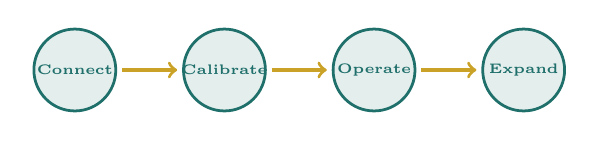
\begin{tikzpicture}[x=1cm, y=1cm]
    \foreach \i/\lbl in {0/Connect, 1.9/Calibrate, 3.8/Operate, 5.7/Expand} {
      \fill[accent!12] (\i,0) circle (0.52);
      \draw[accent, line width=1pt] (\i,0) circle (0.52);
      \node[font=\tiny\bfseries, text=accent] at (\i,0) {\lbl};
    }
    \foreach \i in {0.52, 2.42, 4.32}
      \draw[gold, line width=1.2pt, ->] (\i+0.08,0) -- (\i+0.78,0);
  \end{tikzpicture}
  \end{center}
\end{panel}\hfill
\begin{panel}
  \panelhead{Get in touch}
  \begin{center}
  
\begin{tikzpicture}[scale=1.1]
    \draw[accent, line width=2pt] (0,0) circle (1.05);
    \fill[gold]       (-0.5,-0.5) rectangle (-0.24, 0.05);
    \fill[accent]     (-0.13,-0.5) rectangle ( 0.13, 0.38);
    \fill[accent!60]  ( 0.24,-0.5) rectangle ( 0.5, 0.68);
  \end{tikzpicture}\\[8pt]
  {\Large\bfseries\color{accent}Meridian Analytics}\\[2pt]
  {\small\color{inkgray}Clarity from data.}
  \end{center}

  \vspace{10pt}
  {\small
  {\bfseries\color{accent}Visit}\\
  {\color{inkgray}400 Harbor Street, Suite 210\\
  Portland, OR 97209}\\[7pt]
  {\bfseries\color{accent}Call}\\
  {\color{inkgray}+1 (503) 555-0142, weekdays 8 to 6 PT}\\[7pt]
  {\bfseries\color{accent}Write}\\
  {\color{inkgray}hello@meridiananalytics.example}\\[7pt]
  {\bfseries\color{accent}Online}\\
  {\color{inkgray}meridiananalytics.example}}

  \vspace{12pt}
  {\color{gold}\rule{\linewidth}{1.5pt}}\\[6pt]
  {\small\bfseries\color{accent}Book a 30-minute demo}\\
  {\small\color{inkgray}Bring one quarter of sales history and we will
  show you a working forecast on your own data, free of charge.}
\end{panel}

\end{document}
